%%=============================================================================
%% chapters/chapter3.tex — Automated 3D Mapping (final-defense version)
%%=============================================================================
\chapter{Automated 3D Mapping}
\label{ch:mapping}
This chapter presents the first of the three parts of the framework: automated
3D mapping.\footnote{The content of this chapter is based on the author's ICCAS~2026 paper~\cite{iccas2026} and its journal extension in \emph{Sensors}~\cite{kim2026sensors}.} The subsystem drives a mobile platform carrying a survey-grade
terrestrial laser scanner (TLS) and a complementary onboard 2D laser, acquiring
registered point clouds across an unknown environment while minimizing human
intervention. Because the survey-grade scanner requires stationary acquisition
and does not register scans online, the exploration logic is reformulated
around a stop-and-scan paradigm. Section~\ref{sec:stopscan-arch} states the
problem and the hierarchical architecture; Section~\ref{sec:frontier-layer}
describes the frontier exploration layer; Section~\ref{sec:sequencing}
describes the stop-and-scan sequencer; Section~\ref{sec:coverage} defines the
coverage models on which the scan/skip decision rests and introduces the
occlusion-aware ray-cast visibility model; and Section~\ref{sec:placement}
defines the placement policy built on it. Section~\ref{sec:registration}
closes the chapter with offline registration and the map products handed to
the subsequent parts.

\section{Problem Setting and Architecture}
\label{sec:stopscan-arch}

Automated 3D mapping of indoor and industrial environments with a survey-grade
stationary sensor belongs to what this dissertation calls \emph{robotic
stop-and-scan LiDAR mapping}: a mobile platform carries a sensor that must
remain stationary during each acquisition, and the dense scans are aligned
offline rather than registered incrementally in real time. A TLS is the
canonical instance; the Leica BLK360~G1~\cite{leica-blk360} used in the
experiments acquires a dense colored point cloud from a single viewpoint with a
3D point accuracy on the order of millimeters and a full-dome scan time of a few
minutes. Two properties shape the mapping problem: the sensor must remain
completely stationary during acquisition, and the dense scans are not
registered in real time. Conventional frontier-based exploration, which assumes
continuous motion and online registration, is therefore not directly
applicable. When each stop incurs a sensing cost of minutes, the planner
must decide \emph{where} to stop and scan so that the environment is covered
with as few stationary acquisitions as possible, while preserving the
inter-scan overlap that offline registration requires.

The proposed subsystem decouples high-level exploration from low-level scanning
through a hierarchical architecture (Figure~\ref{fig:mapping-arch}): a
frontier exploration layer continuously proposes navigation goals over a 2D
occupancy grid maintained from the onboard laser, while a stop-and-scan
sequencer monitors displacement, applies a distance gate and a coverage-based
scan/skip decision, and arbitrates when the platform must halt to perform a
survey-grade acquisition. The two layers are coupled through a control service
so that the sequencer can suspend and resume the explorer's active goal. At the
heart of the scan/skip decision is a \emph{coverage model}: a prediction of
which part of the environment a scan pose will actually observe. The
conventional and computationally convenient choice is an isotropic disk model
that treats every free cell within the sensing range as covered. This
assumption is reasonable in open space but fails in the presence of occlusion:
it claims cells that lie within range yet are separated from the sensor by a
wall or partition, judges occluded regions as already covered, and skips the
scans needed to observe them. The visibility model of Section~\ref{sec:coverage}
replaces it. Figure~\ref{fig:dataflow} shows the data flow between the two
layers and its correspondence to the equations of this chapter.

\begin{figure}[!htb]
  \centering
  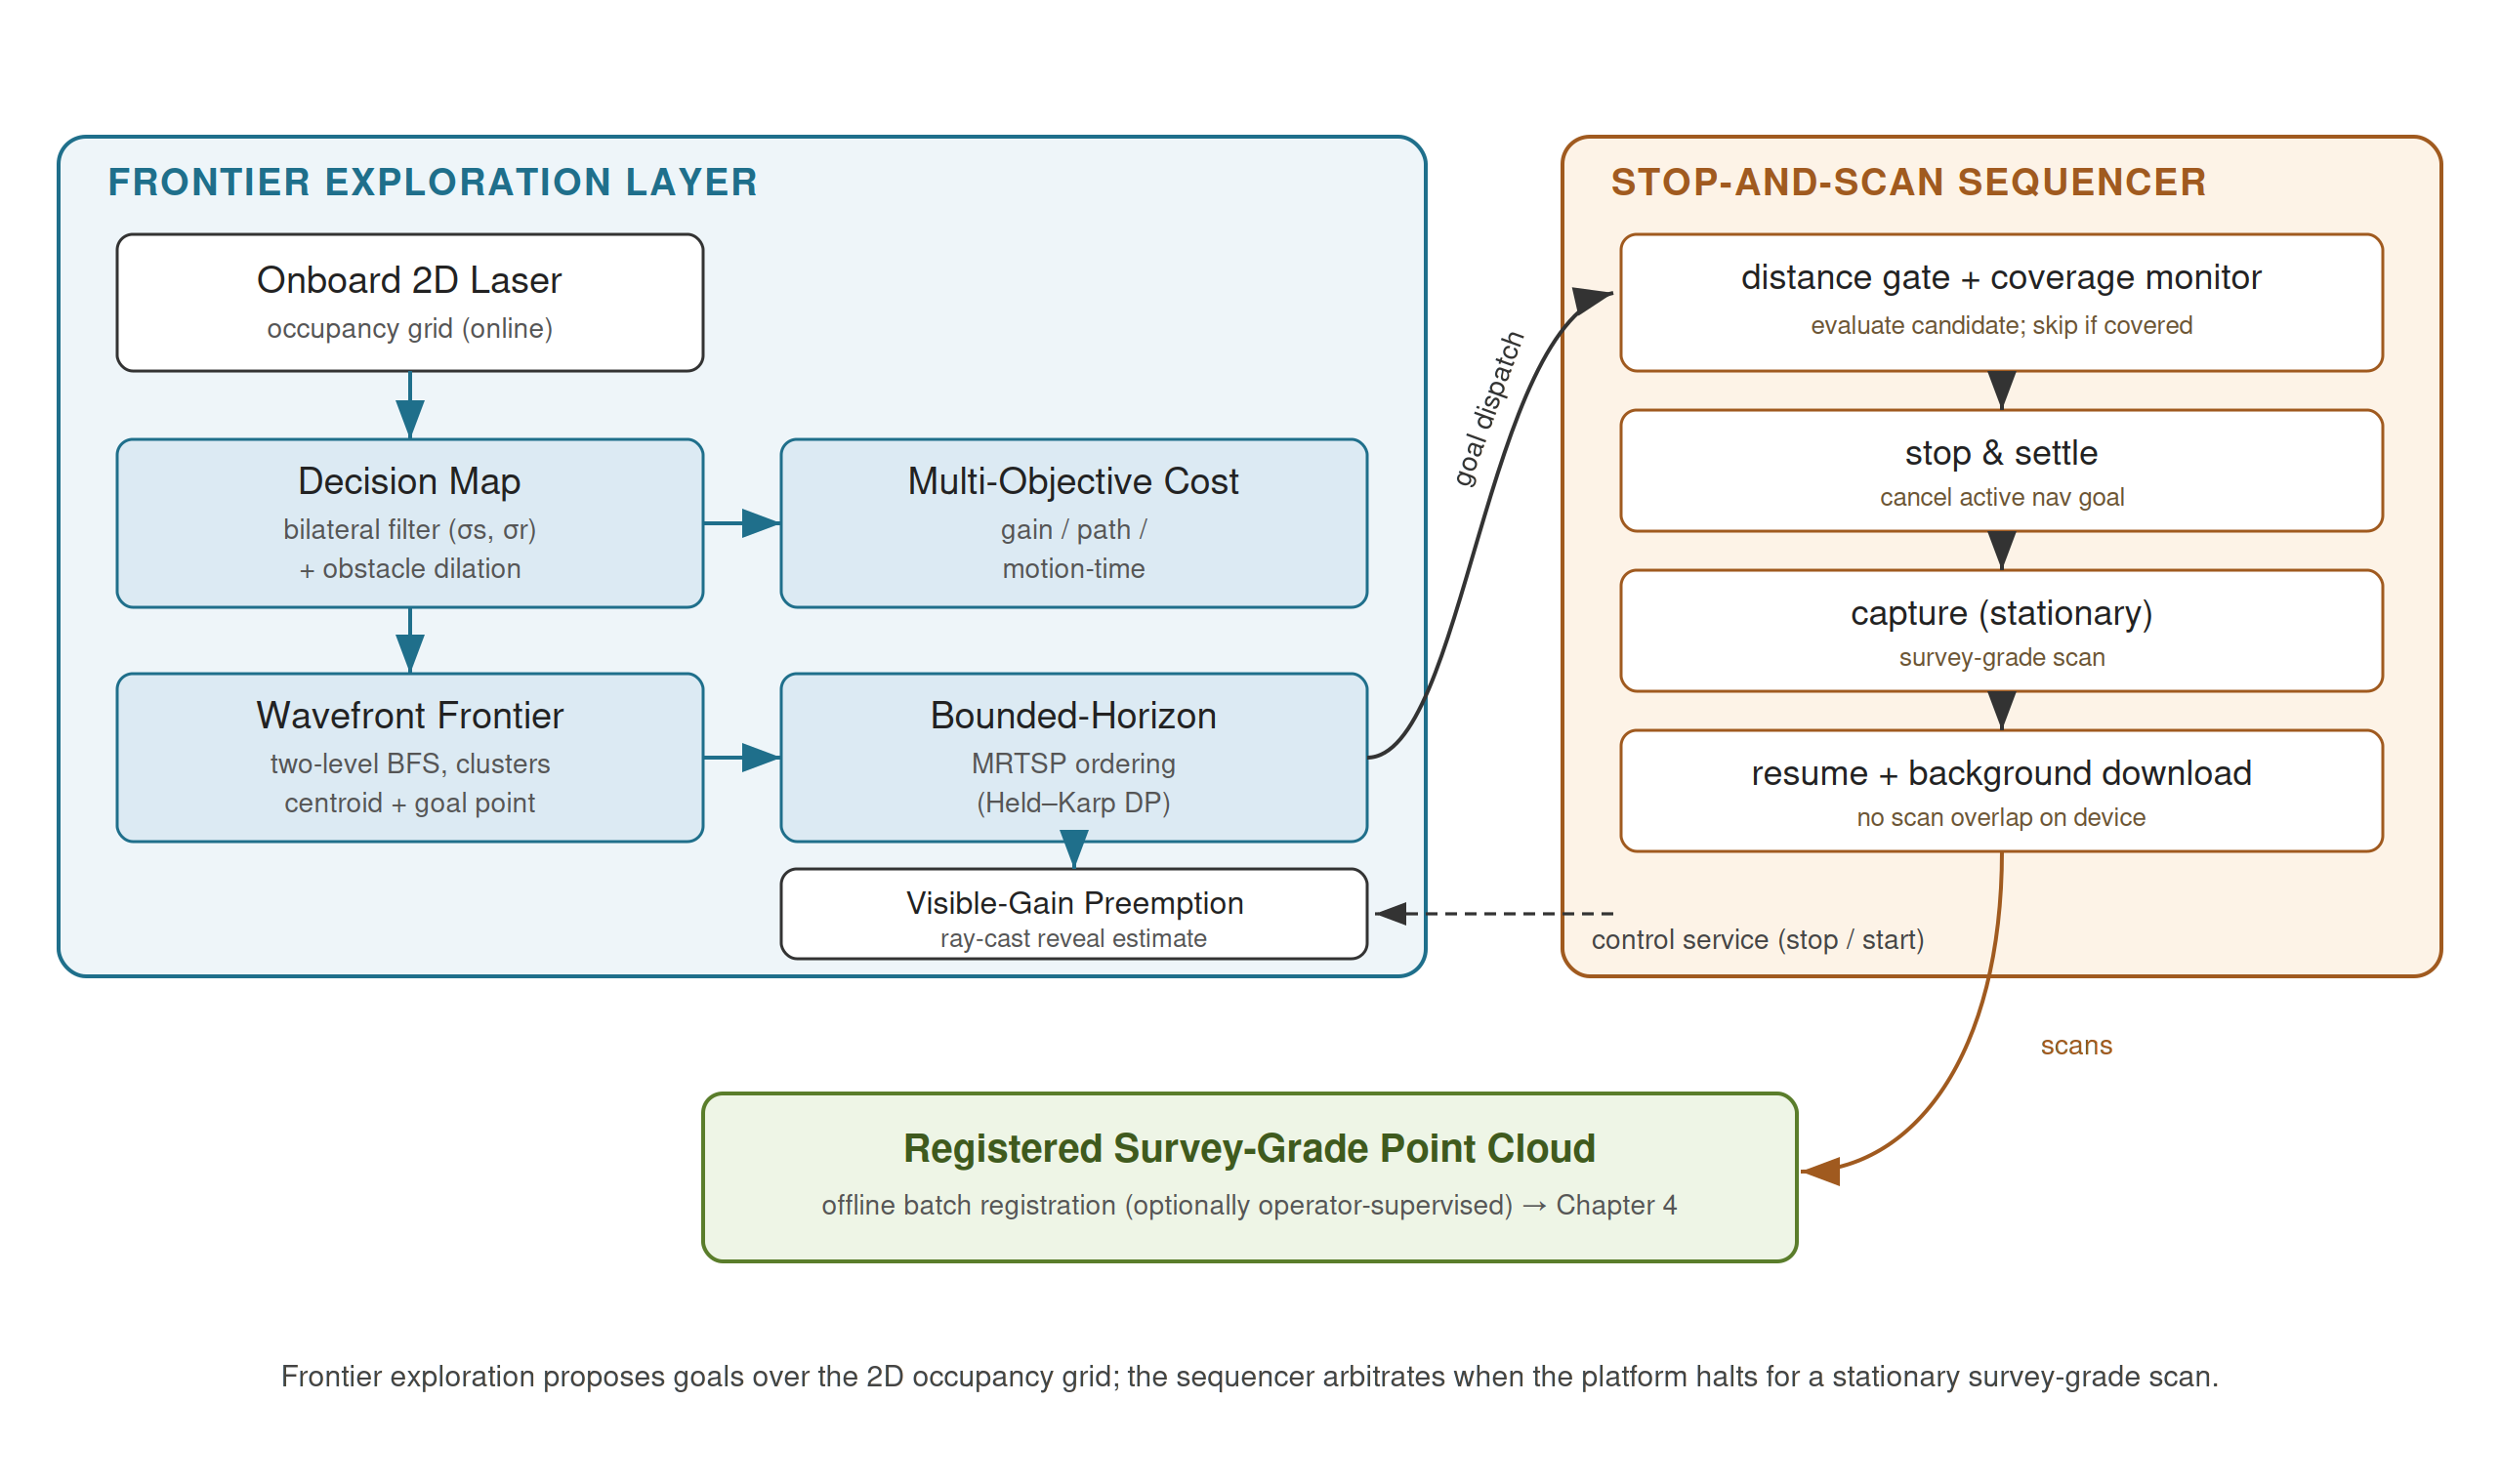
\includegraphics[width=0.95\textwidth]{figures/fig3_1.png}
  \caption{Architecture of the automated 3D mapping subsystem: the frontier
  exploration layer (decision map, wavefront detection, multi-objective cost,
  bounded-horizon ordering) and the stop-and-scan sequencer (distance gate plus
  coverage monitor), coupled through a control service.}
  \label{fig:mapping-arch}
\end{figure}

\begin{figure}[!htb]
  \centering
  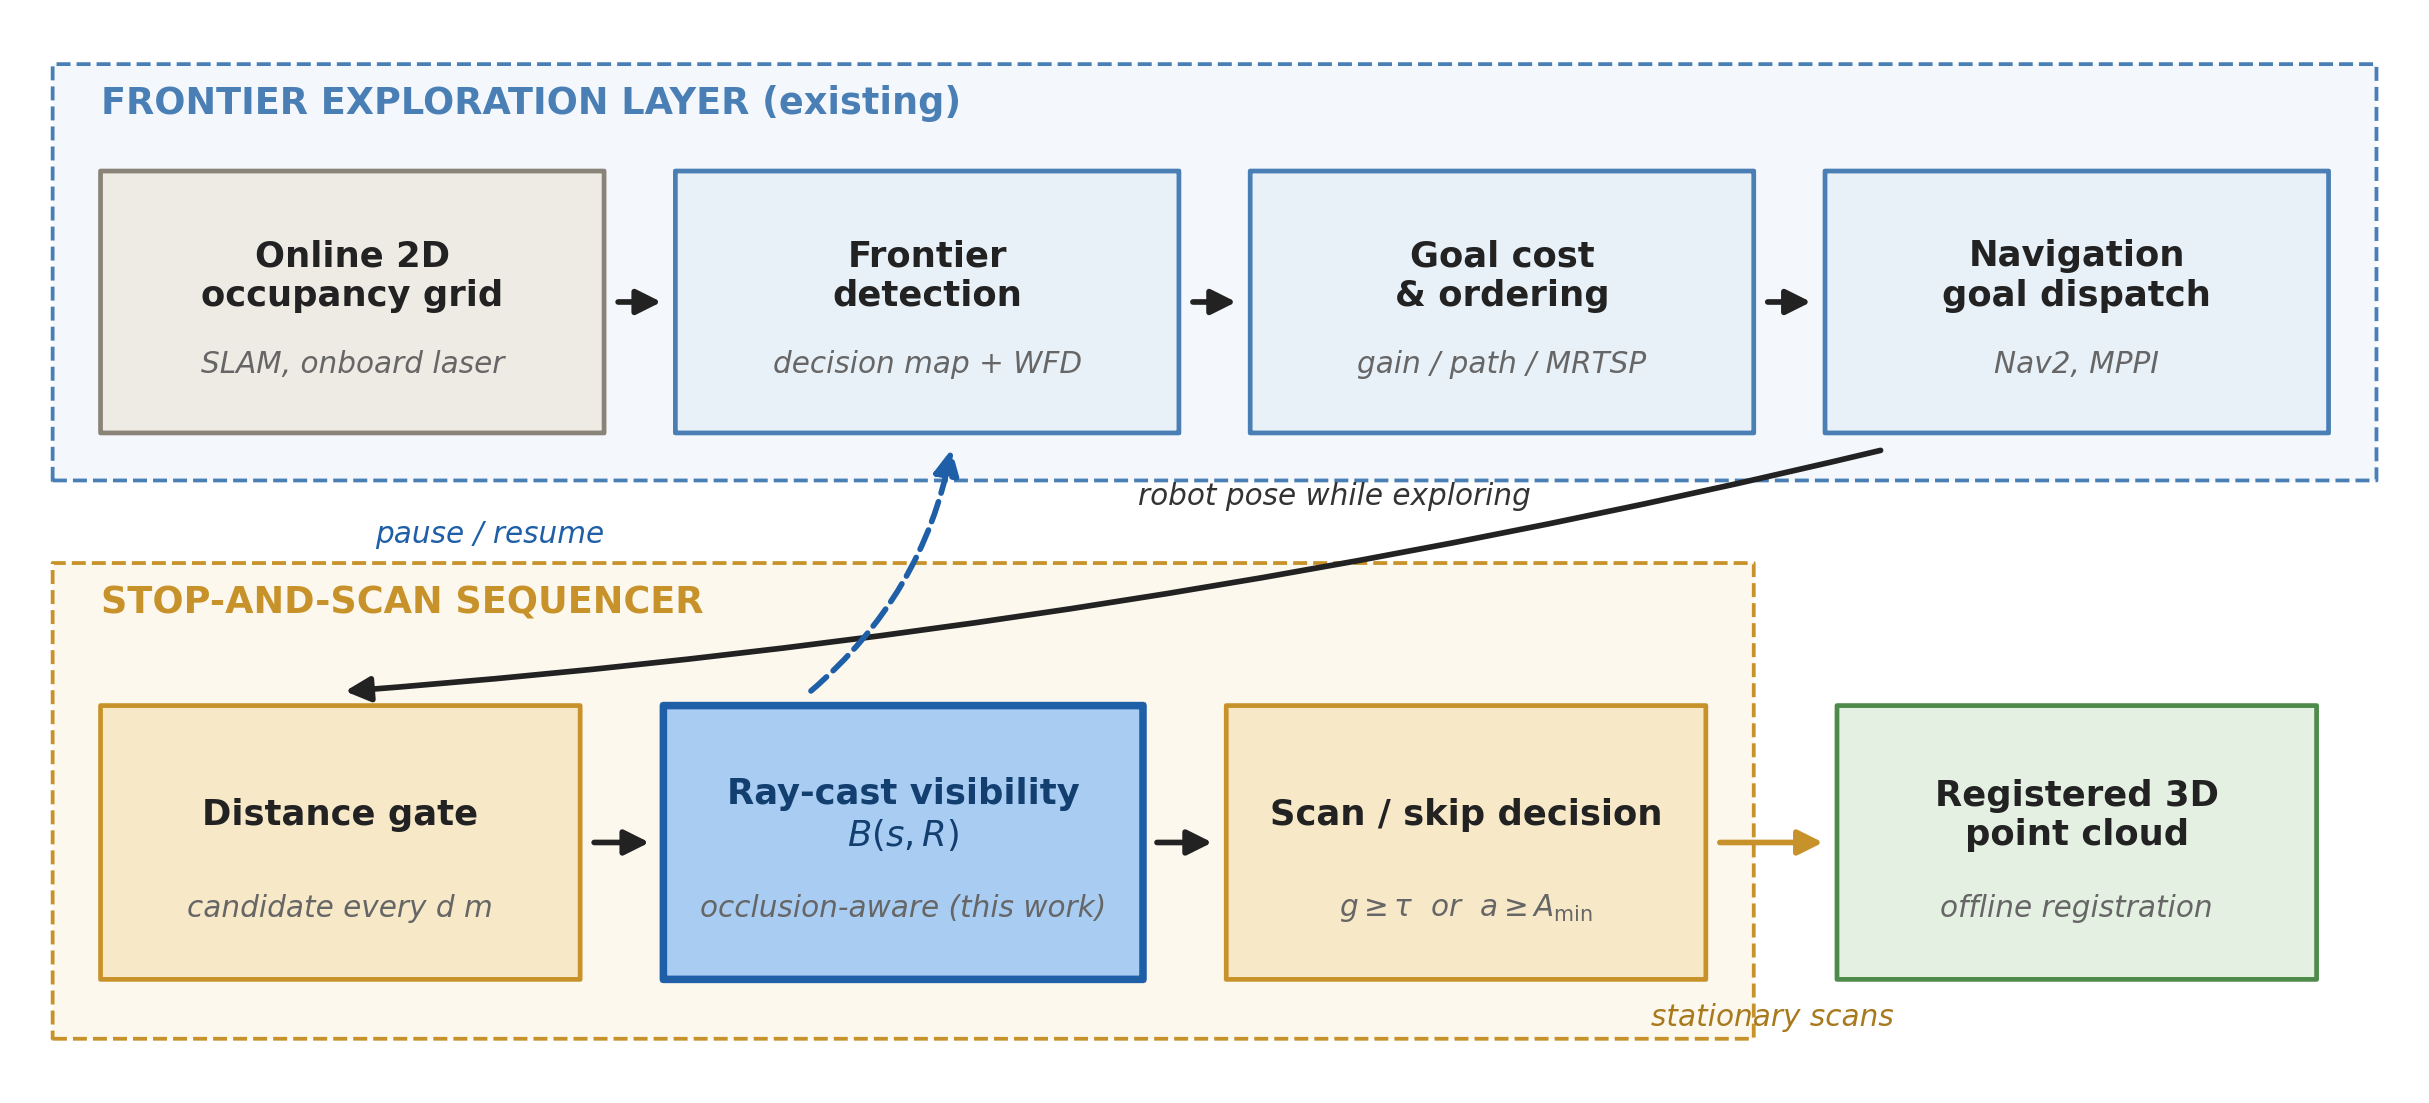
\includegraphics[width=\textwidth]{figures/sen_fig0_architecture.png}
  \caption{Data flow of the stop-and-scan-integrated frontier exploration. The
  exploration layer (top) proposes and orders navigation goals on the live
  occupancy grid; the stop-and-scan sequencer (bottom) applies the
  visibility-based scan/skip rule and triggers stationary scans that are
  registered offline.}
  \label{fig:dataflow}
\end{figure}

\section{Frontier Exploration Layer}
\label{sec:frontier-layer}

The frontier exploration layer is adopted from an open-source ROS~2 frontier
exploration package~\cite{guler2024}; its decision-map construction, wavefront
frontier detection, multi-objective cost, and bounded-horizon visit ordering
are summarized here because the stop-and-scan sequencer and the coverage model
of this dissertation are wrapped around them. The contribution of this work
lies in the stop-and-scan sequencer, the exploration monitor, the coverage
model and placement policy, the BLK360 integration, and the
offline-registration and map-conversion pipeline that orchestrate survey-grade
scans on top of this explorer.

\subsection{Decision Map Construction}
\label{subsec:decision-map}

Raw occupancy grids produced during online navigation contain speckle noise and
ragged unknown-space boundaries that destabilize frontier extraction. Before
frontiers are detected, the raw grid is transformed into a decision map through
an edge-preserving denoising stage. A joint bilateral filter~\cite{tomasi1998}
is applied over the occupancy field, combining a spatial Gaussian kernel of
standard deviation $\sigma_s$ with a range kernel of standard deviation
$\sigma_r$ that distinguishes free, occupied, and unknown cell values; this
suppresses isolated misclassifications while preserving the sharp
free--unknown boundaries on which frontier detection depends. Formally, the
filtered value at cell $p$ is the normalized weighted average over its
neighborhood $N(p)$,
\begin{equation}
  O(p) = \frac{1}{W_p}\sum_{q\in N(p)}
    \exp\!\left(-\frac{\lVert p-q\rVert^2}{2\sigma_s^2}\right)
    \exp\!\left(-\frac{\lvert I(p)-I(q)\rvert^2}{2\sigma_r^2}\right) I(q),
  \label{eq:bilateral}
\end{equation}
where $I(\cdot)$ is the raw occupancy value, $O(\cdot)$ the filtered value, and
$W_p$ the sum of the same weights, which normalizes the result so that the
filter output remains on the scale of the input. The spatial kernel radius is
set to $\lceil 2\sigma_s\rceil$ cells. A subsequent morphological dilation of
obstacles by a structuring element $B_r$ of radius $r$ enforces a conservative
clearance margin,
\begin{equation}
  O_{\mathrm{dil}}(p) = \max_{q\in B_r(p)} O(q),
  \qquad B_r(p)=\{\,q:\lVert p-q\rVert\le r\,\}.
  \label{eq:dilation}
\end{equation}
The filtered decision map is cached and regenerated only when the underlying
grid changes, so that repeated frontier queries on an unchanged map incur no
recomputation.

\subsection{Wavefront Frontier Detection}
\label{subsec:wavefront}

Frontiers---free cells adjacent to unknown space---are extracted from the
decision map using a two-level wavefront breadth-first search. An outer search
expands the navigable free region outward from the robot cell; whenever it
encounters a frontier-eligible cell, an inner search grows the complete
connected frontier cluster to which that cell belongs. Clusters smaller than a
minimum cell count are discarded as noise. For each retained cluster $F$, the
algorithm computes a centroid
\begin{equation}
  c = \frac{1}{\lvert F\rvert}\sum_{i\in F}\mathbf{x}_i,
  \qquad \mathbf{x}_i=(x_i,y_i)\in\mathbb{R}^2,
  \label{eq:centroid}
\end{equation}
used as the ranking reference point, and a representative goal point selected
as the cluster point closest to the centroid that also lies beyond a minimum
goal distance from the robot, ensuring that the dispatched goal is both
representative and reachable. If the robot projects into unknown or occupied
space, a recovery search nudges the seed to the nearest reachable free cell.

\subsection{Multi-Objective Frontier Cost}
\label{subsec:cost}

Each candidate frontier is scored through a multi-objective cost that balances
the information expected from visiting it against the effort required to reach
it. Let the information gain of a candidate be $g=\lvert F\rvert$, its cluster
size. The cost charged to the first dispatched step from the robot pose is
\begin{equation}
  c_{\mathrm{start}} = \frac{w_d\,L_{\mathrm{path}}}{g^{\,w_s}}
    + \frac{t_{\mathrm{motion}}}{\sqrt{g}},
  \label{eq:cstart}
\end{equation}
whereas a frontier-to-frontier transition in the visit sequence is charged the
distance-over-gain term only,
\begin{equation}
  c_{\mathrm{edge}}(i\!\to\! j) =
    \frac{w_d\,L_{\mathrm{path}}(i\!\to\! j)}{g_j^{\,w_s}}.
  \label{eq:cedge}
\end{equation}
Here $w_d$ is the distance weight and $w_s$ the gain exponent. The path length
$L_{\mathrm{path}}$ uses a two-point frontier approximation that discounts the
effective sensor range $r_s$,
\begin{equation}
  L_{\mathrm{path}} = \max(d_m+d_u,\; d_n+d_v) - r_s,
  \label{eq:lpath}
\end{equation}
where $d_m$ and $d_n$ are the distances from the source to the target goal
point and centroid, and $d_u$ and $d_v$ the distances from those two target
points to a start-world reference (Figure~\ref{fig:twopoint}a). The motion-time
lower bound separates translation at maximum linear speed $v_{\max}$ from
in-place rotation toward the target at maximum angular speed $w_{\max}$,
\begin{equation}
  t_{\mathrm{motion}} = \frac{D}{v_{\max}}
    + \frac{\min(\lvert\Delta\psi\rvert,\;2\pi-\lvert\Delta\psi\rvert)}{w_{\max}},
  \label{eq:tmotion}
\end{equation}
where $D$ is the translation distance and $\Delta\psi$ the heading change
required to face the target. Dividing the path term by $g^{w_s}$ and the
motion-time term by $\sqrt{g}$ makes larger, more informative clusters
cheaper, and hence preferred, while nearer candidates of comparable size
remain favored; the
sensor-range discount rewards candidates that extend coverage without redundant
overlap. The relative dominance of the two terms reverses with cluster size at
the crossover $g^*$ defined by
\begin{equation}
  g^{*\,(w_s-1/2)} = \frac{w_d\,L_{\mathrm{path}}}{t_{\mathrm{motion}}},
  \label{eq:crossover}
\end{equation}
so that for small clusters the motion-time term dominates and nearby candidates
are strongly preferred, whereas for large clusters the path term dominates and
coverage extension is rewarded. The gain exponent $w_s$ thus tunes this
crossover size to the high fixed cost of each stationary scan.
Table~\ref{tab:cost-terms} summarizes the terms.

\begin{table}[htbp]
  \centering
  \caption{Terms of the multi-objective frontier cost and their governing
  parameters.}
  \label{tab:cost-terms}
  \begin{tabularx}{\textwidth}{l X l}
    \toprule
    \textbf{Term} & \textbf{Meaning} & \textbf{Governing parameter} \\
    \midrule
    $g=\lvert F\rvert$ & Information gain proxy (frontier cluster size) & minimum frontier size \\
    $L_{\mathrm{path}}$ & Two-point frontier path approximation minus sensor reach & sensor effective range $r_s$ \\
    $t_{\mathrm{motion}}$ & Translation $+$ heading-change lower-bound time & $v_{\max}$, $w_{\max}$ \\
    $w_d$ & Distance weight on the path term & distance weight \\
    $w_s$ & Gain exponent shaping breadth vs.\ economy & gain exponent \\
    \bottomrule
  \end{tabularx}
\end{table}

\subsection{Bounded-Horizon Visit-Order Optimization}
\label{subsec:visit-order}

Selecting only the single cheapest frontier at each step is myopic and can
induce inefficient back-and-forth motion that is especially costly when every
stop incurs a multi-minute scan. The visit order is therefore optimized over a
bounded planning horizon, formulated as a single-platform bounded-horizon
traveling-salesman problem over a cost matrix whose zeroth row and column
represent a synthetic robot start node. Let $dp[S][j]$ denote the minimum cost
of a route that starts at the robot node, visits exactly the set $S$ of
frontiers, and ends at frontier $j\in S$. The Held--Karp~\cite{heldkarp1962}
recurrence is
\begin{equation}
  dp[S\cup\{j\}][j] = \min_{i\in S}\bigl(dp[S][i] + c_{\mathrm{edge}}(i\!\to\! j)\bigr),
  \qquad dp[\{j\}][j] = c_{\mathrm{start}}(j).
  \label{eq:heldkarp}
\end{equation}
The dynamic program expands one path-length layer at a time, so states whose
cardinality exceeds the planning horizon $K$ are never materialized; the
optimal $K$-step route is recovered by following parent pointers backward from
the minimum-cost terminal state. The candidate pool is pruned to a configurable
limit $N$ by $c_{\mathrm{start}}$ before the dynamic program runs, keeping the
bitmask state within a 64-frontier capacity, and a greedy nearest-by-cost
traversal is used as a fallback when the pool exceeds capacity. The number of
materialized states and the time complexity are bounded as
\begin{equation}
  \lvert\text{states}\rvert = \sum_{k=1}^{K}\binom{N}{k}\,k = O(2^K K),
  \qquad \text{time} = O(2^K K^2),
  \label{eq:complexity}
\end{equation}
so keeping $K$ small makes real-time replanning feasible even when each stop
takes several minutes (Figure~\ref{fig:twopoint}b).

\begin{figure}[!htb]
  \centering
  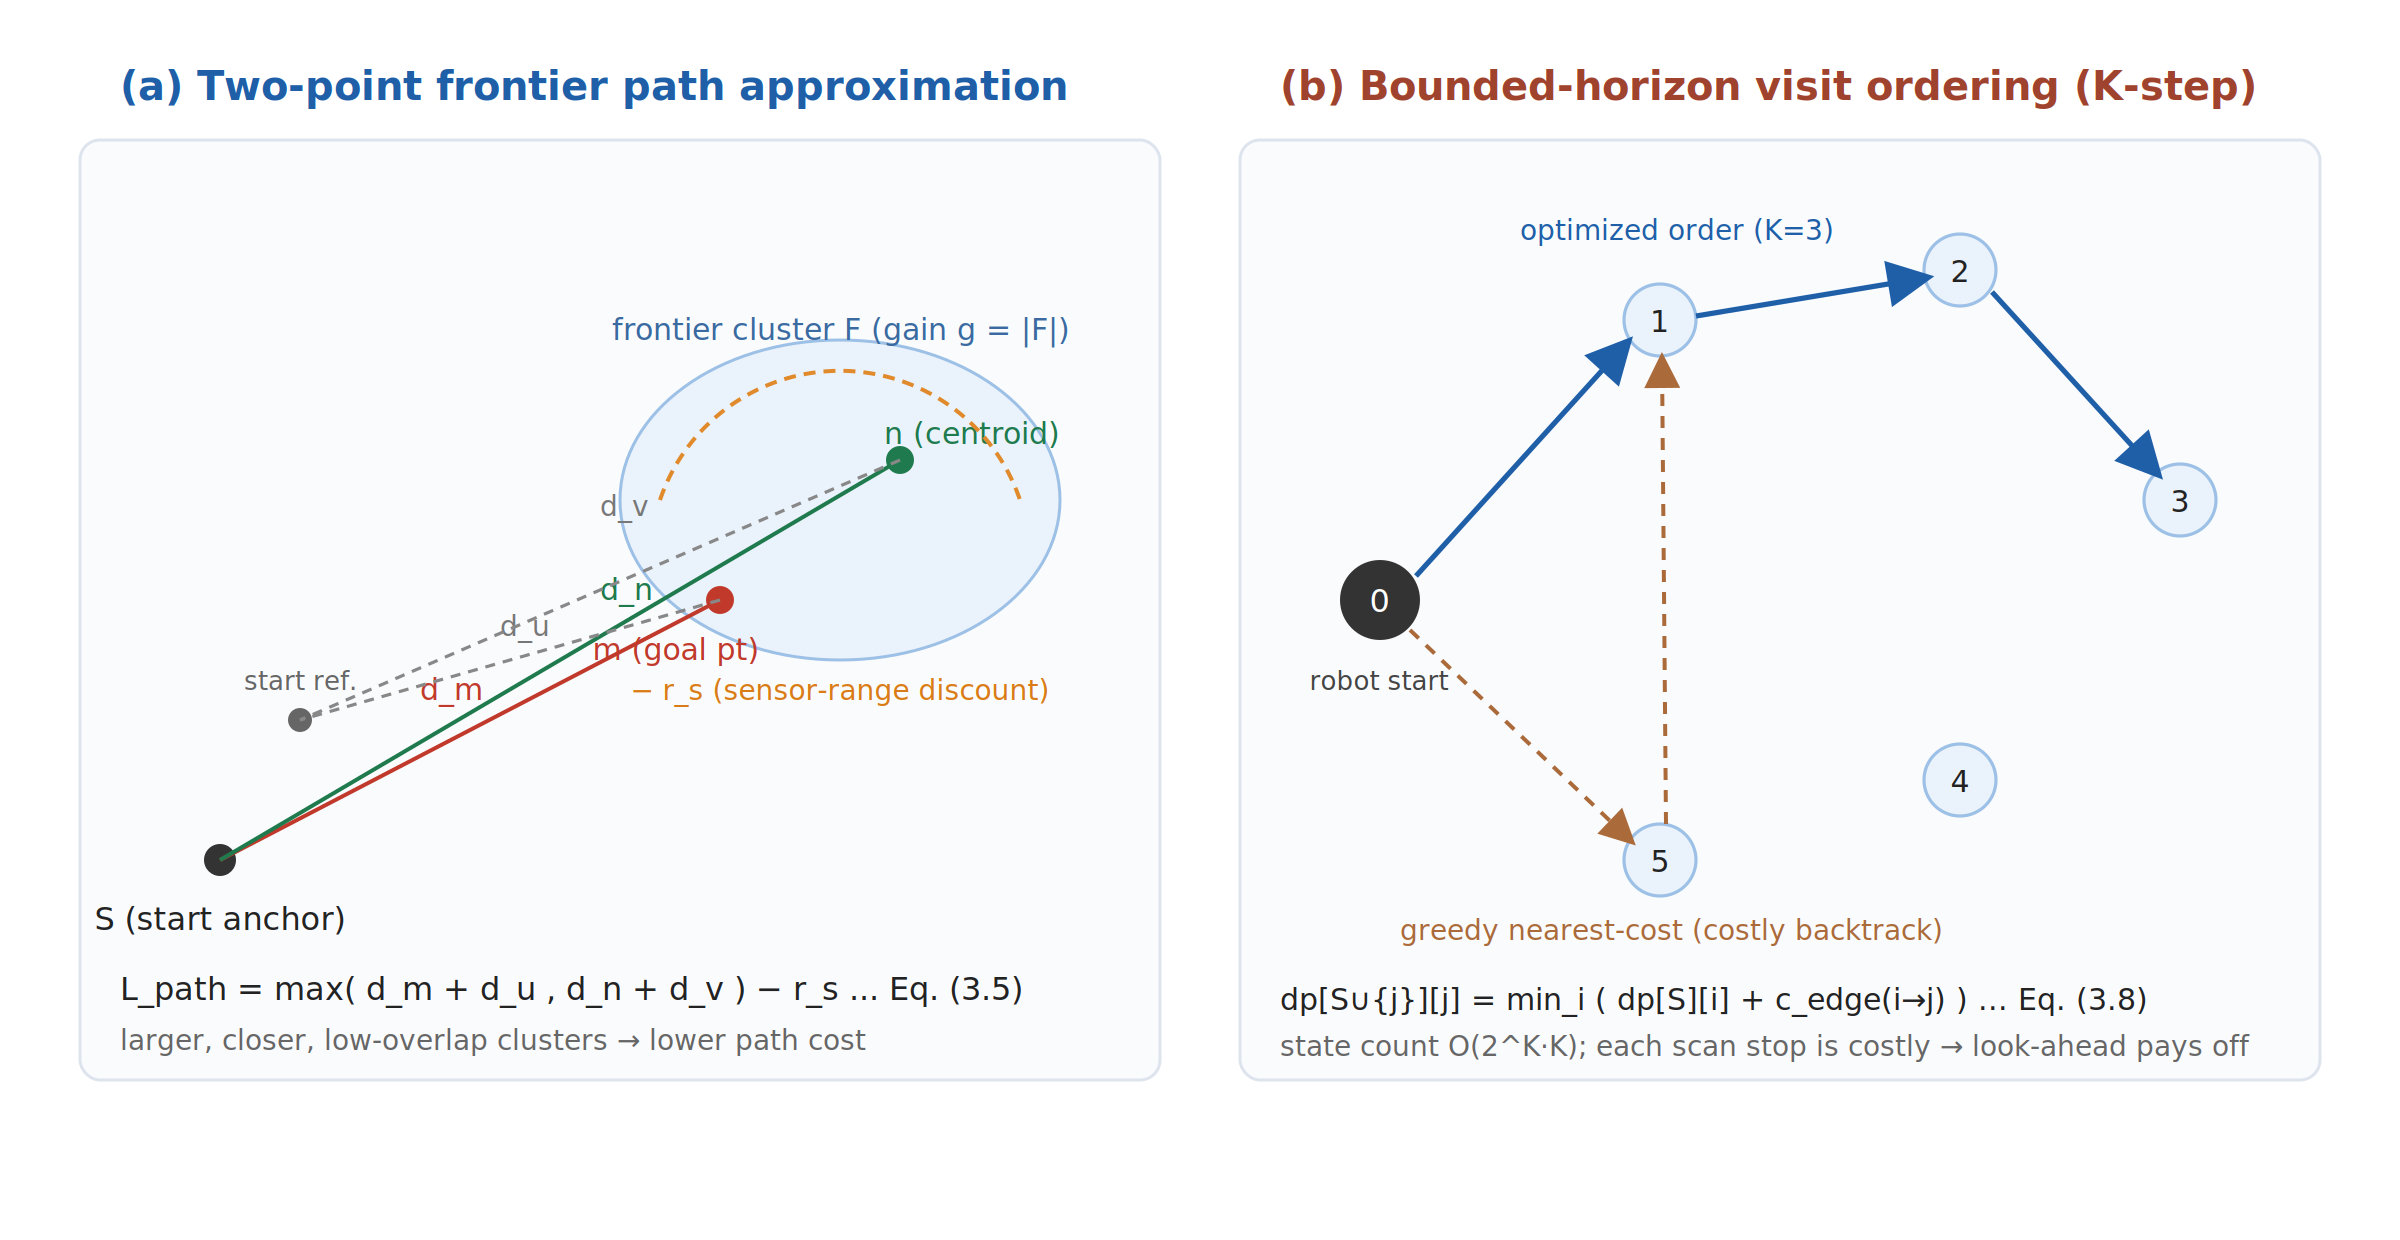
\includegraphics[width=0.92\textwidth]{figures/fig3_4.png}
  \caption{(a) Two-point frontier path approximation
  (Equation~\ref{eq:lpath}): the effective sensor range $r_s$ is discounted
  from the distances to the goal point $m$ and centroid $n$ from the start
  anchor. (b) Bounded-horizon visit ordering (Equation~\ref{eq:heldkarp}):
  because each stationary scan is costly, $K$-step look-ahead reduces the
  backtracking of greedy selection.}
  \label{fig:twopoint}
\end{figure}

\section{Stop-and-Scan Sequencing}
\label{sec:sequencing}

\subsection{Sequencer State Machine}
\label{subsec:fsm}

The stop-and-scan sequencer governs when survey-grade acquisitions occur. It is
structured as a finite-state machine with the states EXPLORING, STOPPING,
SCANNING, RECONNECT, and RESUMING (Figure~\ref{fig:fsm}). During EXPLORING, the
frontier layer drives the platform while the sequencer monitors the net
straight-line displacement of the robot in the map frame from the last
evaluation reference position $q$. A scan \emph{candidate} is raised when
\begin{equation}
  \lVert p_t - q\rVert_2 \ge d,
  \label{eq:distance-gate}
\end{equation}
where $p_t$ is the current platform position and $d$ is the candidate
interval; the reference $q$ is initialized to the start pose and advanced at
every raised candidate whether or not it is accepted. Because this is net displacement rather than path length, dwelling or
circling in place raises no candidate. When a candidate is accepted by the
placement rule of Section~\ref{sec:placement}, the sequencer transitions to
STOPPING, halts the active navigation goal through the control service, and
waits until the platform comes to rest. It then enters SCANNING, triggers a
survey-grade acquisition, and waits for a capture confirmation. Because the
scanner separates a stationary capture phase from a subsequent background
download phase, the sequencer resumes exploration once the capture is
confirmed, allowing the platform to drive toward the next scan point while the
previous scan downloads; two scans are never allowed to overlap on the device,
\begin{equation}
  [\,t_c,\,t_c+\tau_c\,] \,\cap\, [\,t_d,\,t_d+\tau_d\,] = \varnothing,
  \label{eq:no-overlap}
\end{equation}
where $t_c$ and $t_d$ are the capture and download start times and $\tau_c$
and $\tau_d$ the corresponding durations.
Acquisition failures or link drops transition the machine to RECONNECT, which
retries the acquisition up to a bounded number of attempts before either
resuming or aborting.

\begin{figure}[!htb]
  \centering
  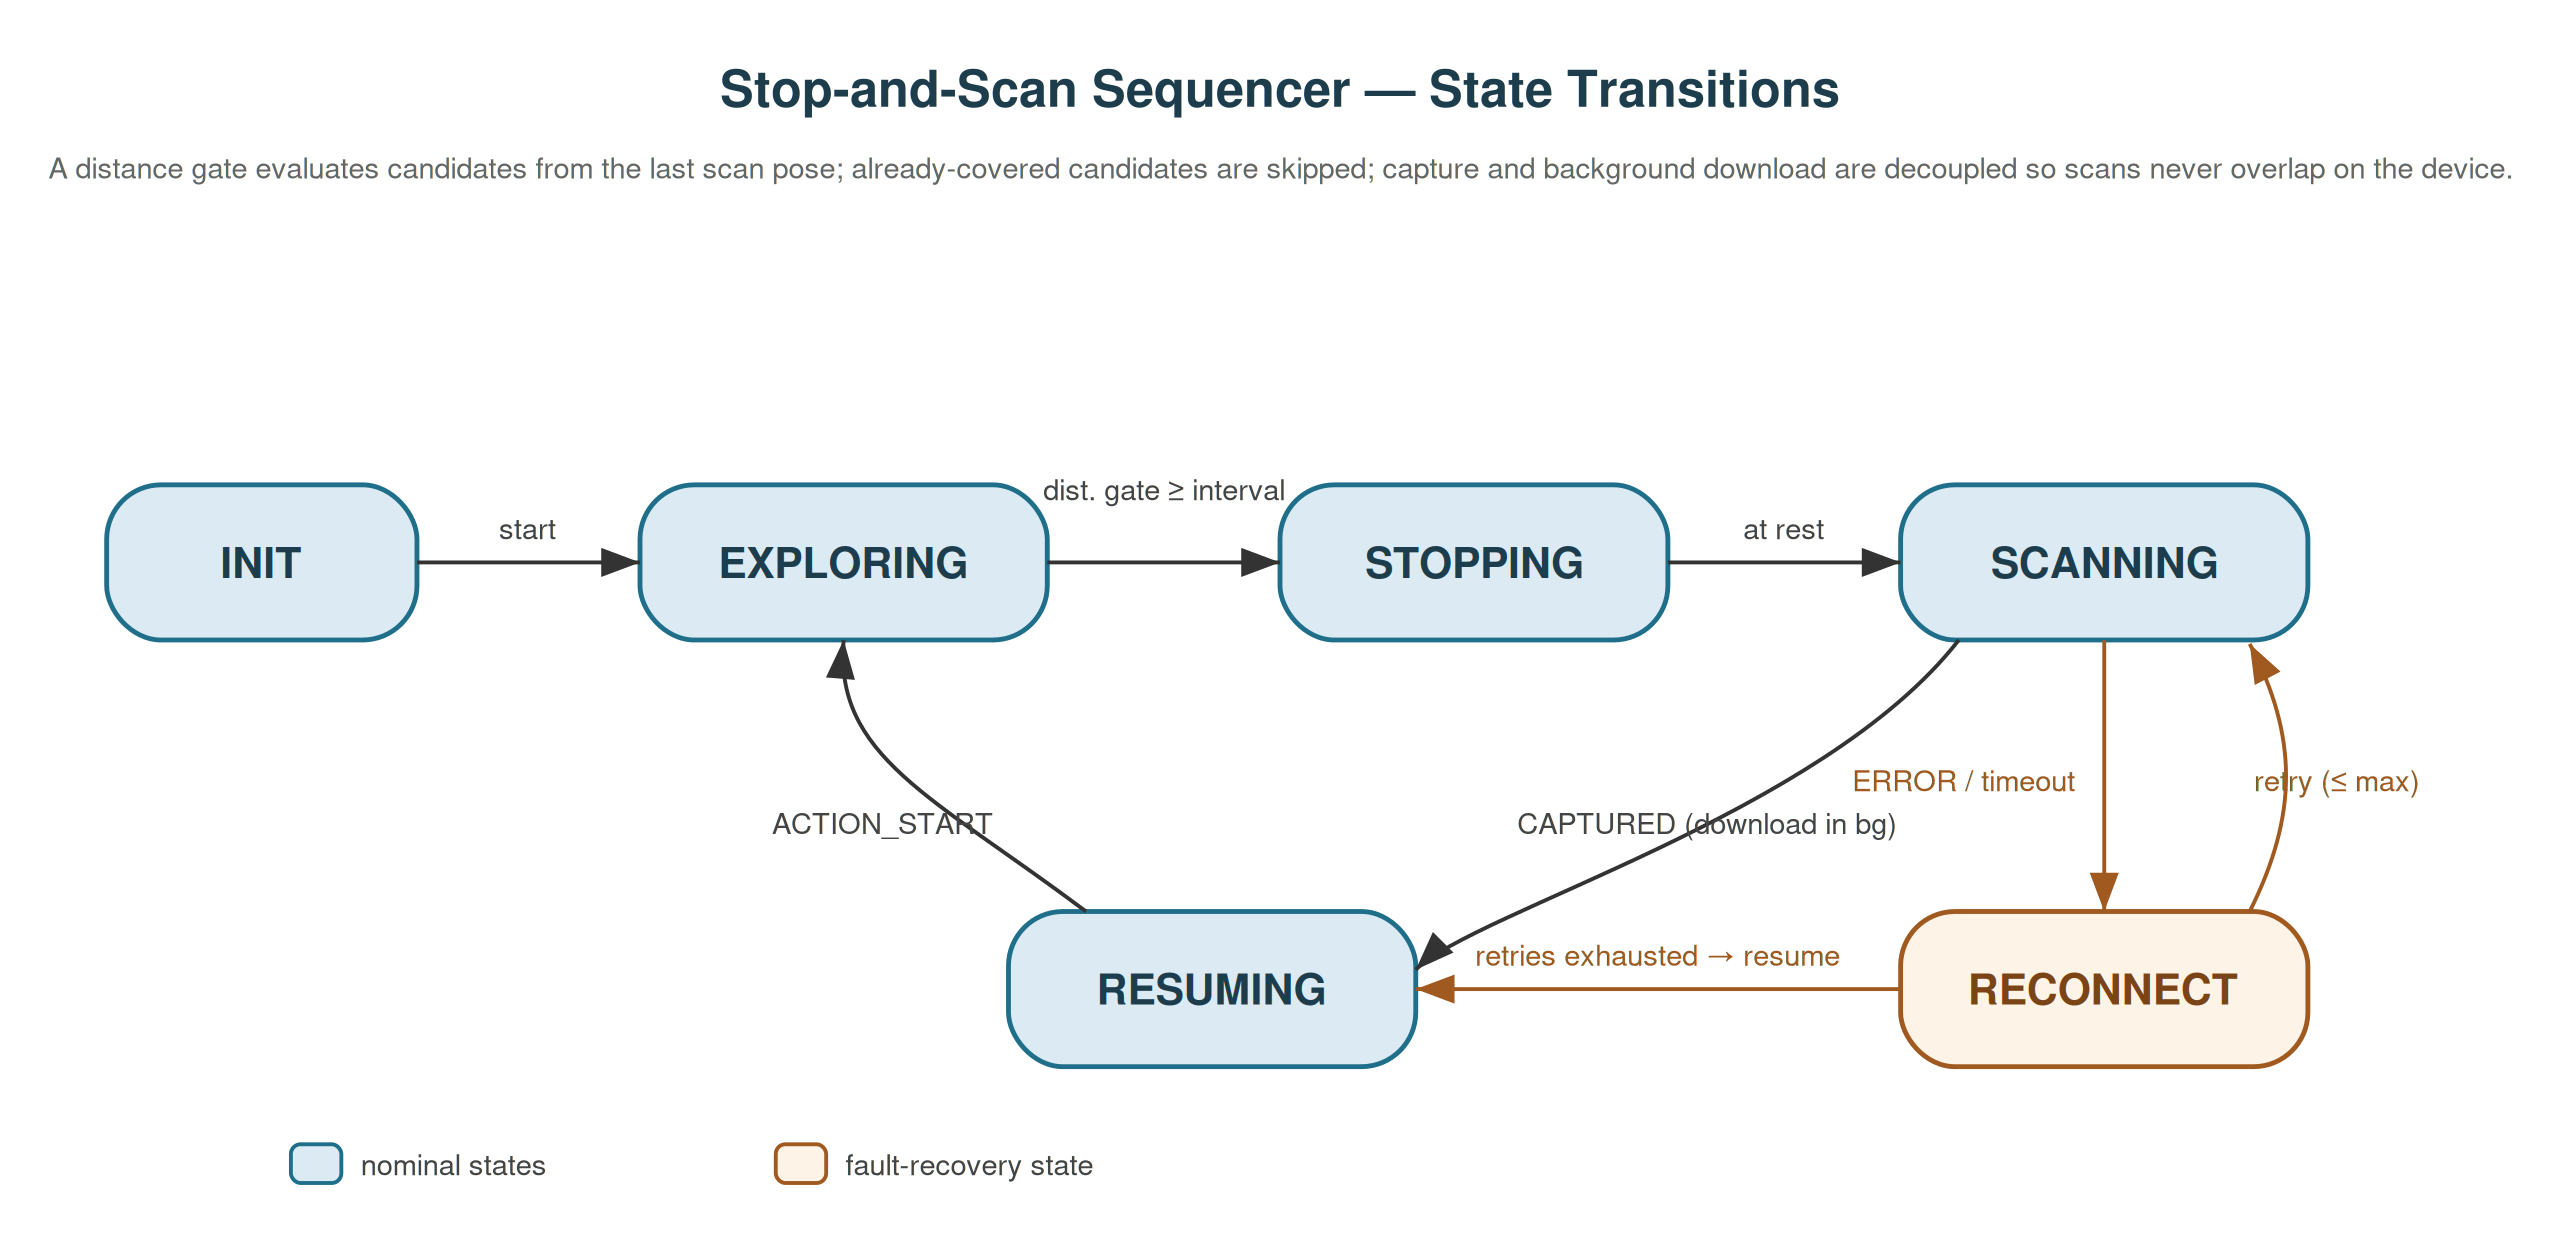
\includegraphics[width=0.95\textwidth]{figures/fig3_2.png}
  \caption{State-transition diagram of the stop-and-scan sequencer: INIT $\to$
  EXPLORING $\to$ STOPPING $\to$ SCANNING $\to$ (RECONNECT) $\to$ RESUMING
  $\to$ EXPLORING, with a distance gate, a coverage-based scan/skip decision,
  and capture--download decoupling.}
  \label{fig:fsm}
\end{figure}

\subsection{Goal Preemption and Frontier Suppression}
\label{subsec:preemption}

During navigation toward a frontier goal, newly revealed map information may
render the active goal redundant before the platform arrives. The subsystem
therefore applies a visible-gain goal-preemption test. Using a ray-casting
sensor model from the prospective goal pose, parameterized by an effective
range, a field of view, and an angular ray step, the subsystem counts how many
genuinely unknown frontier cells would still be revealed from that pose; rays
terminate at occupied cells or at the local cluster bounds, and each revealed
cell is counted at most once,
\begin{equation}
  G_{\mathrm{vis}}(p) = \bigl\lvert\{\,\text{first unknown frontier cell hit by ray }k\,\}\bigr\rvert,
  \qquad L_{\mathrm{reveal}} = G_{\mathrm{vis}}\cdot\Delta r,
  \label{eq:preempt}
\end{equation}
where $\Delta r$ is the map resolution that converts the cell count into a
reveal-length estimate. If $L_{\mathrm{reveal}}$ falls below a threshold, or
the platform is already within a completion radius of the goal, the active
goal is preempted and the next goal in the optimized sequence is dispatched. A
minimum time interval between preemptions prevents goal churn. A complementary
frontier-suppression mechanism temporarily blacklists clusters that repeatedly
fail to make progress, expanding a suppression region around them and pruning
expired suppressions over time, so that the explorer does not fixate on
unreachable frontiers.

\subsection{Exploration Termination}
\label{subsec:termination}

Exploration termination is decided by two independent criteria. The first is
the explorer's native frontier exhaustion: when no reachable, qualifying
frontier remains after suppression and an escape-mode retry, a completion event
is fired. The second is the stall detection of the exploration monitor
implemented in this work: while actively exploring, if the count of known cells
in the occupancy grid grows by less than a minimum progress margin over a fixed
window, the map is treated as converged and termination is declared. The stall
clock is frozen during scan and download pauses so that a long scan is never
mistaken for convergence. This criterion requires no ground truth. The monitor
publishes the remaining frontier count and a latched completion flag, and logs
an end-of-run summary of elapsed time, number of scans, skipped candidates, and
completed downloads; these are the quantities reported in
Section~\ref{sec:exp-mapping}.

\subsection{Proximity-Based Scan/Skip Rule (Baseline)}
\label{subsec:proximity-rule}

The preliminary version of the sequencer~\cite{iccas2026} decided whether to
scan or skip a candidate by a proximity test. Let $S=\{s_1,\dots,s_n\}$ be the
positions actually scanned so far and define the nearest-scan distance of a
candidate position $p$ as $D(p)=\min_{s_i\in S}\lVert p-s_i\rVert_2$ (with
$D(p)=+\infty$ when $S=\varnothing$). The rule scans when $D(p)\ge R$ and skips
when $D(p)<R$, where $R$ is an effective coverage radius set with reference to
the scanner's range; equivalently, it skips whenever the candidate falls inside
the union of disks of radius $R$ around previous scans. This is the
\emph{disk spacing rule} of stop-and-go practice. It is retained in this
dissertation as the baseline against which the visibility-based rule is
evaluated, and Section~\ref{subsec:prelim-mapping} reports the scan-trigger
comparison that first motivated a coverage-based skip decision at all: without
any redundancy check, a distance-traveled trigger fires a stationary scan at
every travel interval and maps the test room with seven times more scans than
necessary.

\section{Coverage Models for Stop-and-Scan Placement}
\label{sec:coverage}

This section defines the coverage model at the core of the scan/skip decision.
The workspace is formalized on an occupancy grid, the isotropic disk model is
contrasted with the proposed ray-cast visibility region, and the line-of-sight
coverage metric is defined.

\subsection{Workspace and Notation}
\label{subsec:notation}

Let the environment be represented by a 2D occupancy grid~\cite{elfes1989,thrun2005}
$\mathcal{M}$ produced online by SLAM. The grid is an $H\times W$ array of
square cells of side $\rho$ (the grid resolution, $\rho=0.05$~m in all
experiments); each cell $c$ is identified with its center point in the map
frame. Each cell carries an integer value $o(c)$, where $o(c)=-1$ denotes
unmapped space and $o(c)\in[0,100]$ is a scaled occupancy probability. Cells
are classified as
\begin{equation}
\mathrm{state}(c)=
\begin{cases}
\textit{free}, & 0 \le o(c) \le \theta_{\mathrm{free}}, \\
\textit{occupied}, & o(c) \ge \theta_{\mathrm{occ}}, \\
\textit{unknown}, & o(c)=-1 \ \text{or}\ \theta_{\mathrm{free}}<o(c)<\theta_{\mathrm{occ}},
\end{cases}
\label{eq:state}
\end{equation}
with $\theta_{\mathrm{free}}=25$ and $\theta_{\mathrm{occ}}=65$, the
long-standing free/occupied convention of the ROS occupancy-map
pipeline~\cite{macenski2020marathon}. The classification is insensitive to the
exact placement of these values because SLAM-estimated occupancies are strongly
bimodal. The two thresholds are deliberately separated: a cell is treated as
free only when its occupancy is confidently low and as an obstacle only when
confidently high; the intermediate band is treated as unknown so that ambiguous
cells are neither counted as covered nor allowed to pass a sight line. The
set of mapped free cells, the region over which coverage is evaluated, is
written $\mathcal{F}=\{c\in\mathcal{M}:\mathrm{state}(c)=\textit{free}\}$. A
\emph{scan pose} is a stationary viewpoint $s_i\in\mathcal{F}$ at which the
platform halts and the stop-and-scan sensor acquires data; each sensor is
characterized by a range bound $R$ out to which its visibility region is
evaluated. Throughout, $s_i$ denotes an accepted scan pose, $p$ a candidate
pose under evaluation, and $c$ a grid cell.

\subsection{Isotropic Disk Coverage (Baseline)}
\label{subsec:disk}

A widely adopted and computationally convenient assumption is that a scan pose
covers every free cell within its range, giving the \emph{isotropic disk}
model
\begin{equation}
B_{\mathrm{disk}}(s_i,R)=\{c\in\mathcal{F}:\lVert c-s_i\rVert \le R\}.
\label{eq:disk}
\end{equation}
The disk model depends only on the range bound, is trivial to evaluate, and
is adequate in open, obstacle-free space. Its defining limitation is that it
ignores occlusion: because membership depends solely on proximity,
$B_{\mathrm{disk}}$ claims cells within range $R$ that are separated from $s_i$
by a wall or partition, i.e., cells to which the sensor has no line of sight
(Figure~\ref{fig:concept}a). At the placement stage, a rule that trusts
$B_{\mathrm{disk}}$ treats such a region as satisfied and skips the scan that
genuine observation would require.

\begin{figure}[!htb]
\centering
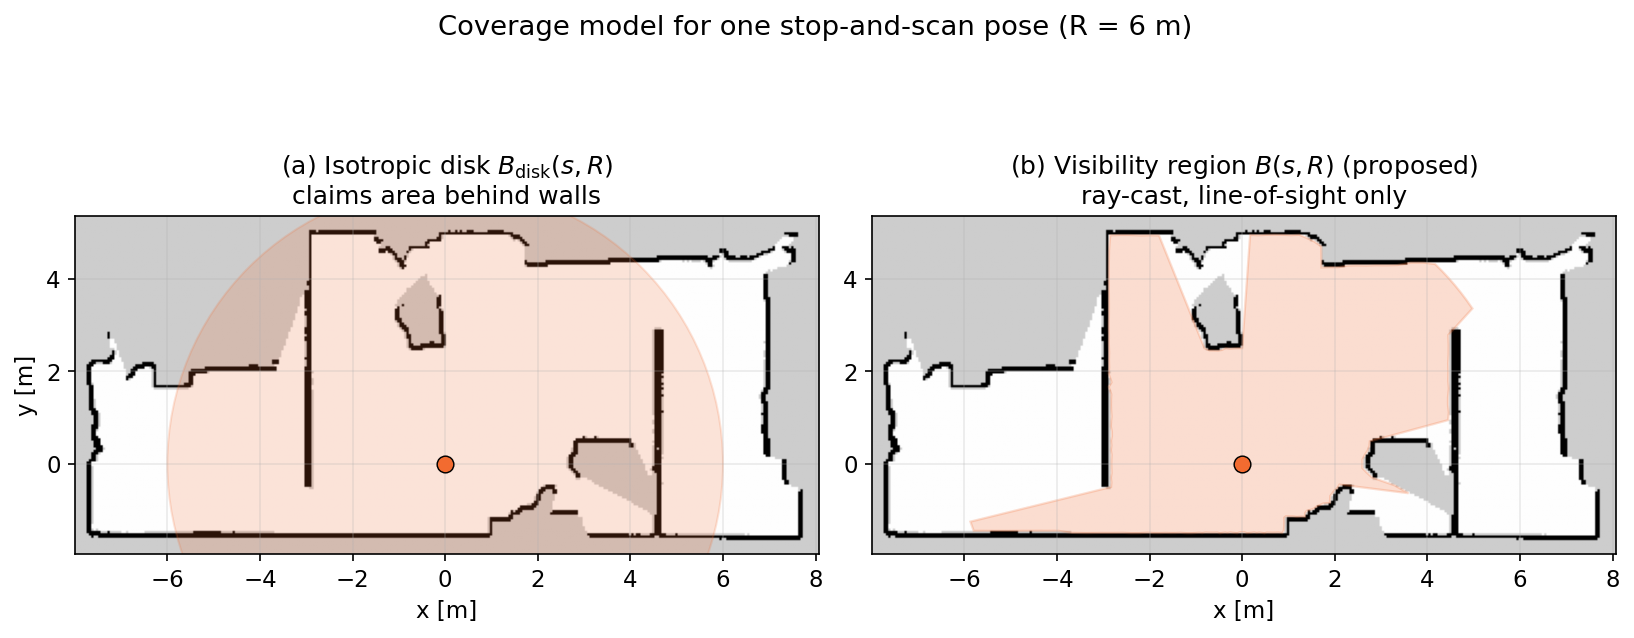
\includegraphics[width=0.85\linewidth]{figures/sen_fig1_concept.png}
\caption{Coverage models for a single scan pose ($R=6$~m). (a)~The isotropic
disk $B_{\mathrm{disk}}(s,R)$ counts every free cell within range as covered,
bleeding through walls. (b)~The proposed ray-cast visibility region $B(s,R)$
claims only genuine line-of-sight area.}
\label{fig:concept}
\end{figure}

\subsection{Ray-Cast Visibility Region (Proposed)}
\label{subsec:visibility}

To account for occlusion, the disk is replaced with a \emph{ray-cast
visibility region}, a discrete visibility polygon that admits only cells in
direct line of sight of the scan pose. From $s_i$, $N_r=720$ rays are cast over a
full $360^\circ$ field at uniform angular resolution
$\Delta\theta=0.5^\circ$. Each ray is marched outward in steps of half a cell
and is truncated at the first sample that is either occupied or unknown; that
terminating cell and everything beyond it on the ray are excluded. Formally,
for a free cell $c$ on the ray at azimuth $\theta_k$, let $\overline{s_i c}$
denote the cells strictly between $s_i$ and $c$ along the ray. Then
\begin{equation}
B(s_i,R)=\left\{c\in\mathcal{F}:
\lVert c-s_i\rVert \le R \ \wedge\
\mathrm{state}(c')=\textit{free}\ \ \forall\, c'\in\overline{s_i c}\right\}.
\label{eq:visibility}
\end{equation}
A free cell is claimed as covered only if every intervening cell along the
sight line to it is also mapped free space. Occupied cells terminate the ray
because the obstacle blocks the beam, and unknown cells terminate it because
the model refuses to assert visibility through unmapped space. This second
condition is deliberately conservative: the model never ``sees through''
regions the map cannot vouch for. The set definition characterizes the ideal
geometric visibility region and does not depend on the ray discretization; the
$K$ rays and half-cell marching are the implementation that approximates it. At
the range bound the inter-ray arc spacing is $R\,\Delta\theta\approx5.2$~cm for
$R=6$~m, on the order of a single grid cell, so the discrete approximation
recovers the ideal region up to single-cell effects at region boundaries. By
construction $B(s_i,R)\subseteq B_{\mathrm{disk}}(s_i,R)$ for any pose and
range: ray-casting can only remove cells the disk would have claimed, and the
two coincide only for an obstacle-free disk around $s_i$
(Figure~\ref{fig:concept}b). Each visibility polygon is computed in pure array
operations in roughly 2~ms, inexpensive enough to evaluate at every scan
candidate online.

\subsection{Line-of-Sight Coverage Metric}
\label{subsec:los}

Coverage by a set of scan poses is the union of their visibility regions. For
$S=\{s_1,\dots,s_n\}$ the covered area is $C(S)=\bigcup_{i=1}^{n} B(s_i,R)$,
and the \emph{line-of-sight (LOS) coverage} is the fraction of mapped free
space observed from at least one scan pose,
\begin{equation}
\mathrm{LOS}(S)=\frac{\lvert C(S)\cap\mathcal{F}\rvert}{\lvert\mathcal{F}\rvert}\in[0,1],
\label{eq:los}
\end{equation}
where $\lvert\cdot\rvert$ counts cells. The complement $1-\mathrm{LOS}(S)$
corresponds to mapped free cells that remain occluded from every scan pose.
Because the metric is defined over $\mathcal{F}$ and visibility never
propagates through occupied or unknown cells, LOS coverage is a conservative
measure of genuine observation rather than the optimistic proximity count
produced by the disk model. It is the single figure of merit reported for
scan placement in Section~\ref{sec:exp-mapping}.

\subsection{Scope: 2D Station Planning for 3D Mapping}
\label{subsec:scope2d}

The visibility model and the LOS metric are deliberately 2D: they
reason on the live occupancy grid, a horizontal slice of the environment at the
mapping sensor's height. LOS coverage therefore certifies sight lines to
floor-space cells, not to the full 3D surface set the scanner observes.
Vertical occlusions---shelves, overhanging structures, elevated machinery, or
surfaces stacked at different heights above the same floor cell---are not
represented, and high 2D LOS coverage does not by itself guarantee complete 3D
surface coverage. This scope is a design choice matched to the online setting:
the occupancy grid is what SLAM makes available in real time on the platform;
the 2D visibility polygon is cheap enough to evaluate at every candidate; and
in the room-scale indoor environments targeted here, a pose with unobstructed
2D line of sight to a floor region generally also observes much of the
structure above it, because the scanner acquires a full dome. The contribution
should accordingly be read as occlusion-aware 2D scan-station planning for
subsequent 3D mapping; a genuinely 3D visibility representation is future work
(Chapter~\ref{ch:conclusion}).

\section{Visibility-Based Placement Policy}
\label{sec:placement}

Section~\ref{sec:coverage} defined what a scan pose observes; this section
defines where the robot decides to stop and scan. Because each stationary scan
carries a large fixed cost, the placement policy must take as few scans as
possible while maintaining high LOS coverage (Equation~\ref{eq:los}) of the
mapped free space.

\subsection{Marginal Visibility Gain}
\label{subsec:gain}

Let $S=\{s_1,\dots,s_n\}$ be the scans accepted so far and
$C(S)=\bigcup_i B(s_i,R)$ their union coverage. The visibility regions of
previously accepted scans are not frozen: at every decision, $C(S)$ is
recomputed on the current occupancy map, so earlier regions expand or contract
as SLAM refines the map. For a candidate pose $p$ raised by the distance gate
(Equation~\ref{eq:distance-gate}), the decision is based on how much \emph{new}
line-of-sight area its visibility region contributes relative to what it sees
in total. The \emph{normalized marginal gain} and the \emph{absolute new
area} are
\begin{equation}
g(p\mid S)=\frac{\lvert B(p,R)\setminus C(S)\rvert}{\lvert B(p,R)\rvert},
\qquad
a(p\mid S)=\lvert B(p,R)\setminus C(S)\rvert\cdot\rho^2,
\label{eq:gain}
\end{equation}
with $g\in[0,1]$ and $a$ in m$^2$. Both quantities are evaluated directly on
the visibility regions, so occlusion is respected: area behind a wall is never
part of $B(p,R)$ and never inflates either the coverage or the gain. A
candidate whose visibility region is degenerate (smaller than 0.5~m$^2$, which
occurs when the pose projects into an obstacle or an unmapped pocket) is
rejected outright before the gain is evaluated, so the denominator never
vanishes.

\subsection{Dual-Criterion Accept/Skip Rule}
\label{subsec:dual}

A naive policy would accept a candidate whenever its relative gain exceeds a
threshold, $g\ge\tau$. This single relative test is fragile for a
room-scale stop-and-scan sensor: because $R$ is comparable to the size of a
room, $B(p,R)$ is large, so a small but genuinely occluded pocket
contributes only a tiny fraction of that region and fails the relative test,
even though it is exactly the kind of unscanned area the method exists to
capture. A candidate is therefore accepted when \emph{either} a relative
\emph{or} an absolute criterion is met,
\begin{equation}
\textsf{scan}(p)\iff
\big(g(p\mid S)\ge\tau\big)\ \lor\ \big(a(p\mid S)\ge A_{\min}\big),
\label{eq:dual}
\end{equation}
and skipped only when both fail. The relative term $\tau$ captures candidates
that open a large new area such as a previously unseen room; the absolute term
$A_{\min}$ rescues small but real occlusion pockets whose new area is a
negligible fraction of the scanner's footprint. The experiments use
$\tau=0.30$ and $A_{\min}=5$~m$^2$ with range bound $R=6$~m;
Section~\ref{subsec:exp-sensitivity} shows that coverage and scan count are
nearly flat in $\tau$ over $[0.10,0.50]$, whereas $A_{\min}$ is the operative
knob trading coverage against scan count, with its knee at 5~m$^2$.

Two disk-based baselines are evaluated against this rule. The first is the
proximity spacing rule of Section~\ref{subsec:proximity-rule}. This rule is
\emph{not} mathematically equivalent to the marginal-gain rule applied to
$B_{\mathrm{disk}}$---a candidate closer than $R$ to an existing scan can still
contribute a crescent of new disk area---so a comparison against it changes
both the coverage model and the acceptance rule. To isolate the coverage model
itself, the ablation of Section~\ref{subsec:exp-ablation} additionally
evaluates a \emph{disk marginal-gain} baseline that applies the identical dual
criterion (Equation~\ref{eq:dual}) with $B_{\mathrm{disk}}$ substituted for
$B$; within that pair, the only difference is the coverage model.

\subsection{Coverage-Completion Phase}
\label{subsec:completion}

Frontier-driven exploration terminates when the known map stops growing
(Section~\ref{subsec:termination}), but convergence of the \emph{map} does not
by itself guarantee that every mapped free cell has been brought into line of
sight: small occluded pockets can remain. The method therefore includes an
optional coverage-completion phase that runs after exploration converges. The
uncovered free cells $\mathcal{F}\setminus C(S)$ are clustered into connected
pockets; for each pocket of area at least $A_{\mathrm{pocket}}$, the robot
navigates into the pocket and takes a stationary scan, repeating until no
qualifying pocket remains. The phase is bounded by per-pocket navigation
timeouts, an overall scan budget, and a list of pockets found unreachable, so
it always terminates. The method does not claim 100\% LOS coverage:
sub-$A_{\mathrm{pocket}}$ fragments at wall and obstacle edges are reported as
residual rather than rounded up.

\subsection{Integration with Exploration}
\label{subsec:integration}

The placement policy is embedded in the autonomous exploration loop without
owning the navigation goals. The frontier explorer drives the robot toward
unmapped space on the live occupancy map; the sequencer monitors displacement,
applies the accept/skip rule at each raised candidate, and triggers a stationary
scan when a candidate is accepted, resuming exploration afterward. Completion
is declared by the exploration monitor, after which the optional
coverage-completion phase runs and the run is finalized.
Algorithm~\ref{alg:placement} summarizes the complete placement policy.

\begin{algorithm}[H]
\caption{Visibility-based stop-and-scan placement}
\label{alg:placement}
\begin{algorithmic}[1]
\Require live occupancy map $\mathcal{M}$; range bound $R$; thresholds $\tau$, $A_{\min}$, $A_{\mathrm{pocket}}$; candidate interval $d$
\Ensure set of accepted scan poses $S$
\State $S \gets \varnothing$;\quad $q \gets$ start pose
\While{exploration not converged}
  \State drive toward frontier goal on $\mathcal{M}$
  \If{$\lVert \mathrm{pose} - q \rVert_2 \ge d$}
    \State $p \gets \mathrm{pose}$;\quad $q \gets p$
    \State $B(p,R) \gets \textsc{RayCastVisibility}(\mathcal{M}, p, R)$
    \If{$\lvert B(p,R)\rvert \cdot \rho^2 < 0.5$} \textbf{continue} \Comment{degenerate pose: skip}
    \EndIf
    \State $g \gets \lvert B(p,R)\setminus C(S)\rvert / \lvert B(p,R)\rvert$;\quad
           $a \gets \lvert B(p,R)\setminus C(S)\rvert \cdot \rho^2$
    \If{$g \ge \tau$ \textbf{or} $a \ge A_{\min}$}
      \State stop and acquire stationary scan at $p$;\quad $S \gets S \cup \{p\}$
    \EndIf
  \EndIf
\EndWhile
\While{$\exists$ pocket $P \subseteq \mathcal{F}\setminus C(S)$ with $\mathrm{area}(P) \ge A_{\mathrm{pocket}}$ and $P$ reachable} \Comment{coverage completion (optional)}
  \State navigate into $P$;\quad acquire scan at reached pose $p$;\quad $S \gets S \cup \{p\}$
\EndWhile
\State \Return $S$
\end{algorithmic}
\end{algorithm}

\section{Offline Registration and Map Products}
\label{sec:registration}

The full 3D registration of the acquired scans is performed as an offline
batch process after the run, optionally under operator supervision when the
scale or complexity of the environment requires it. In this work the BLK360
scans of each run are registered as an independent project in the vendor's
registration software using cloud-to-cloud alignment without artificial
targets; importing and aligning one run's network takes minutes on a desktop
workstation, which is small compared with the acquisition time of the scans
themselves.
The registration report of each network---the number of setups, the number of
pairwise links, the overall overlap, and the bundle-adjustment error---is the
survey-grade product against which the placement policy is ultimately judged
(Section~\ref{subsec:exp-registration}); placement that keeps successive
stations in mutual line of sight yields the pairwise overlaps that
cloud-to-cloud registration requires. The registered cloud is exported as a
single E57 file, which is the input to the semantic modeling of
Chapter~\ref{ch:semantic} and to the scan-to-simulation conversion of
Chapter~\ref{ch:validation}, while the exploration occupancy grid built online
by SLAM is retained as the robot-facing navigation map and as the drift-free
structural prior used by the structure filters of Chapter~\ref{ch:semantic}.

Table~\ref{tab:params} lists the principal parameters of the mapping
subsystem. Values in the upper block are the operating point used in all
experiments unless otherwise noted; values in the lower block are tuned per
environment.

\begin{table}[htbp]
  \centering
  \caption{Principal parameters of the automated 3D mapping subsystem.}
  \label{tab:params}
  \begin{tabularx}{\textwidth}{l l X}
    \toprule
    \textbf{Parameter} & \textbf{Value} & \textbf{Description} \\
    \midrule
    Range bound $R$ & 6~m & Maximum distance out to which the visibility region $B(s,R)$ is evaluated. \\
    Relative threshold $\tau$ & 0.30 & Minimum fraction of new visible area for the relative accept criterion. \\
    Absolute threshold $A_{\min}$ & 5~m$^2$ & Minimum new visible area for the absolute accept criterion. \\
    Candidate interval $d$ & 3~m & Net straight-line displacement between successive scan candidates. \\
    Ray count $N_r$ & 720 & Number of rays per visibility computation ($\Delta\theta=0.5^\circ$). \\
    Free / occupied thresholds & 25 / 65 & Occupancy values bounding mapped free space and ray-terminating obstacles. \\
    Degenerate cut & 0.5~m$^2$ & Minimum visibility-region area; smaller candidates are rejected. \\
    Stop-settle timeout & 8~s & Maximum wait for the platform to come fully to rest before scanning. \\
    Scan timeout / max retries & 240~s / 5 & Capture time limit and reconnection attempts before resume or abort. \\
    \midrule
    Scan-and-download time & env.-tuned & Capture-plus-download duration of the (mock or physical) scanner. \\
    Bilateral-filter std.\ dev. & env.-tuned & Spatial and range kernel widths for decision-map construction. \\
    Obstacle dilation radius & env.-tuned & Morphological dilation enforcing a clearance margin. \\
    Minimum frontier size & env.-tuned & Frontier clusters smaller than this are discarded as noise. \\
    Sensor effective range, $w_d$, $w_s$ & env.-tuned & Cost-term parameters of Section~\ref{subsec:cost}. \\
    Planning horizon $K$, pool size $N$ & env.-tuned & Bounded-horizon ordering parameters ($N\le64$). \\
    Completion pocket area $A_{\mathrm{pocket}}$ & env.-tuned & Minimum uncovered-pocket area triggering a completion scan. \\
    \bottomrule
  \end{tabularx}
\end{table}
